Since $ABCD$ is a parallellogram,
\begin{align}
  \label{eq:chapters/10/7/2/6/tables/det2f}
 \myvec{4 \\y } - \myvec{1 \\2 }  
= \myvec{x \\6 } - \myvec{3 \\5 }  
\\
\implies	\myvec{3\\y-2}=\myvec{x-3\\1}\\
	\text{ or, }x=6 ,y=3.
\end{align}
See  \figref{fig:chapters/10/7/2/6/Fig3}.
\begin{figure}[h!]
	\begin{center}
  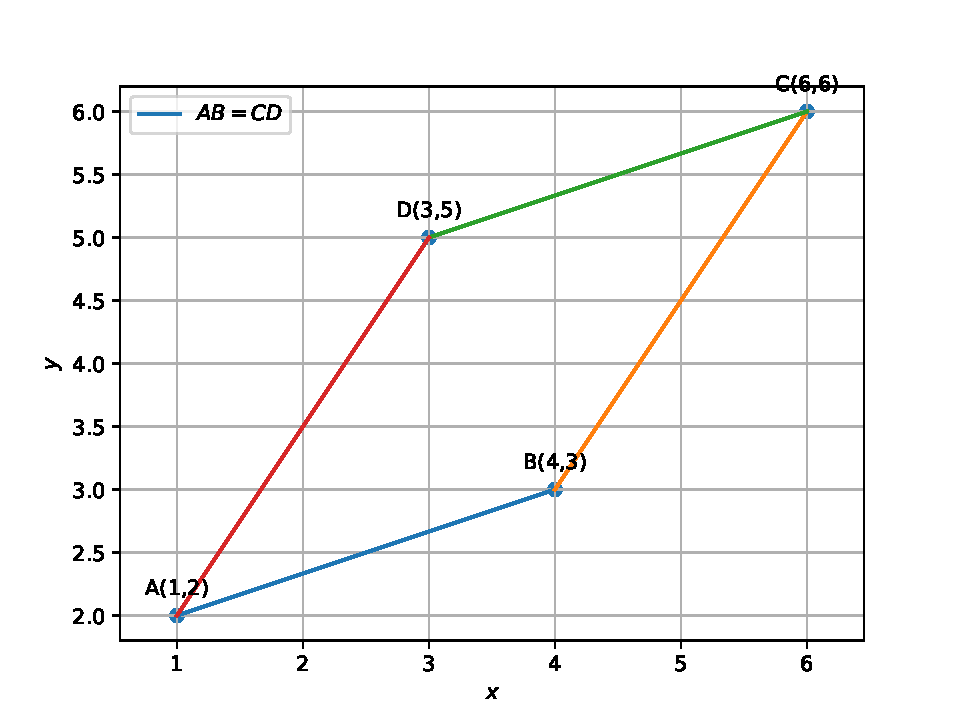
\includegraphics[width=\columnwidth]{chapters/10/7/2/6/figs/para.pdf}
	\end{center}
\caption{}
\label{fig:chapters/10/7/2/6/Fig3}
\end{figure}

